% documentclass
% set font size=11 (11pt)
% set paper format=A4 (a4paper)
% set equation alignment to left (fleqn)
\documentclass[11pt,a4paper,fleqn]{article}


% Preamble
% use the inputenc and fontenc packages to use French accents
\usepackage[utf8]{inputenc}
\usepackage[T1]{fontenc}
% for matrices / vectors
\usepackage{amsmath}
% for references
\usepackage{hyperref}
% allow for arbitrary font size
\usepackage{anyfontsize}
% for color
\usepackage{xcolor}
% for pseudocolor
\usepackage{algorithm,algpseudocode}
% for code samples
\usepackage{listings}
% set the font as Time New Roman (the Latex equivalent, at least)
% \usepackage{mathptmx}
% set the size of the document margins using the geometry package
\usepackage[lmargin=0.97in,rmargin=0.97in,tmargin=1.4in,bmargin=1.4in]{geometry}
% turn the color of footnote markers to black
\renewcommand\thefootnote{\textcolor{black}{\arabic{footnote}}}
% suppress indents on footnotes
\usepackage[hang,flushmargin]{footmisc}
% automatically generates colored brackets around references
\usepackage{fncylab} \labelformat{equation}{(#1)}
% supress indent on new paragraphs
\setlength{\parindent}{0pt}
% use the amsmath package to include mathematical symbols
\usepackage{amsmath}
% suppress the space between the left margin and the equations (fleqn still leaves some space by default)
\setlength{\mathindent}{0pt}
% create a new environment to left flush the equation with the align environment
\makeatletter
\newenvironment{lflalign}{ \vspace{-3mm}%
  \def\align@preamble{%
    &\strut@
    \setboxz@h{\@lign$\m@th\displaystyle{####}$}%
    \ifmeasuring@\savefieldlength@\fi
    \set@field
    \hfil
    \tabskip\z@skip
    &\setboxz@h{\@lign$\m@th\displaystyle{{}####}$}%
    \ifmeasuring@\savefieldlength@\fi
    \set@field
    \hfil
    \tabskip\alignsep@
  }
  \flalign}
{\endflalign}
\makeatother
% use the ammssymb package to use mathematical symbols
\usepackage{amssymb}
% create new commands for mathematical symbols
\DeclareMathOperator{\N}{\mathbb{N}}
\DeclareMathOperator{\Z}{\mathbb{Z}}
\DeclareMathOperator{\Q}{\mathbb{Q}}
\DeclareMathOperator{\R}{\mathbb{R}}
\DeclareMathOperator{\Pb}{\mathbb{P}}
% declare the cmsy (computer modern symbol) math alphabet to define appropriate fonts for the U and N mathematical symbols
\DeclareMathAlphabet\mathbcal{OMS}{cmsy}{m}{n}
% create new commands for mathematical symbols
\DeclareMathOperator{\E}{\mathbcal{E}}
\DeclareMathOperator{\Ex}{\mathbb{E}}
\DeclareMathOperator{\F}{\mathbcal{F}}
\DeclareMathOperator{\G}{\mathbcal{G}}
\DeclareMathOperator{\M}{\mathbcal{M}}
\DeclareMathOperator{\HH}{\mathbcal{H}}
\DeclareMathOperator{\QQ}{\mathbcal{Q}}
\DeclareMathOperator{\PP}{\mathbcal{P}}
\DeclareMathOperator{\Noo}{\mathbcal{N}}
\DeclareMathOperator{\U}{\mathbcal{U}}
% use the bbm package to be able to use the double stroke 1 for the indicator function
\usepackage{bbm}
\DeclareMathOperator{\ind}{\mathbbmss{1}}
% use the bm package to use bold characters in math mode
\usepackage{bm}
% create a new command for black square bullets
\newcommand{\bs}{\scalebox{0.7}{$\blacksquare$} \hspace{2mm}}
% use the relsize package to be abe to change the size of mathematical symbols
\usepackage{relsize}
% define a new command for in-line small summation
\newcommand{\ssumm}[2]{\underset{\scriptscriptstyle #1}{\overset{\scriptscriptstyle #2}{\mathlarger{\mathlarger{\mathlarger{\Sigma}}}}} \hspace{0.5mm}}
% define a new command for in-line small products
\newcommand{\sprod}[2]{\underset{\scriptscriptstyle #1}{\overset{\scriptscriptstyle #2}{\mathlarger{\mathlarger{\mathlarger{\Pi}}}}} \hspace{0.5mm}}
% Use the caption package to customize captions (titles) of tables and graphs
\usepackage[font=small,labelfont=bf]{caption}
% use float package to force figure the be positioned where indicated
\usepackage{float}
% use the graphicx package to be able to resize tables
\usepackage{graphicx}


\begin{document}

% command to check unused bibliography entries
% \nocite{*}

\section{Intro}

Neural networks became increasingly popular in the last few years as showed by the \href{https://www.kdnuggets.com/2021/05/winning-machine-learning-competition.html}{research publication topics}. The main advantage of those models is that they can learn complex structures and are highly customizable. However, one significant drawback is their poor explanability power. Neural networks are often categorized in the so-called "black box models".
Fortunately, there are some very good tutorials on understanding how a neural network actually works. Today, every data scientist knows the tutorials of \href{https://www.coursera.org/learn/neural-networks-deep-learning}{Andrew Ng}. \\

After having done those tutorials, I personally found out that a 1-layer network is relatively easy to understand, however it gets tricky when increasing the number of layers. This article is an attempt to understand in details the 2-layer neural network through the building of a small playground. We will even publish the playground online! To enjoy fully this article, the reader must be familiar with the working of a 1-layer neural network.\\

There are already an elephantic number of articles on the maths behind neural networks, so I will focus more on the building app as I believe is less frequent. \\

The difference between a 1-layer network and a 2-layer network relies in the following picture: \\

\begin{center}
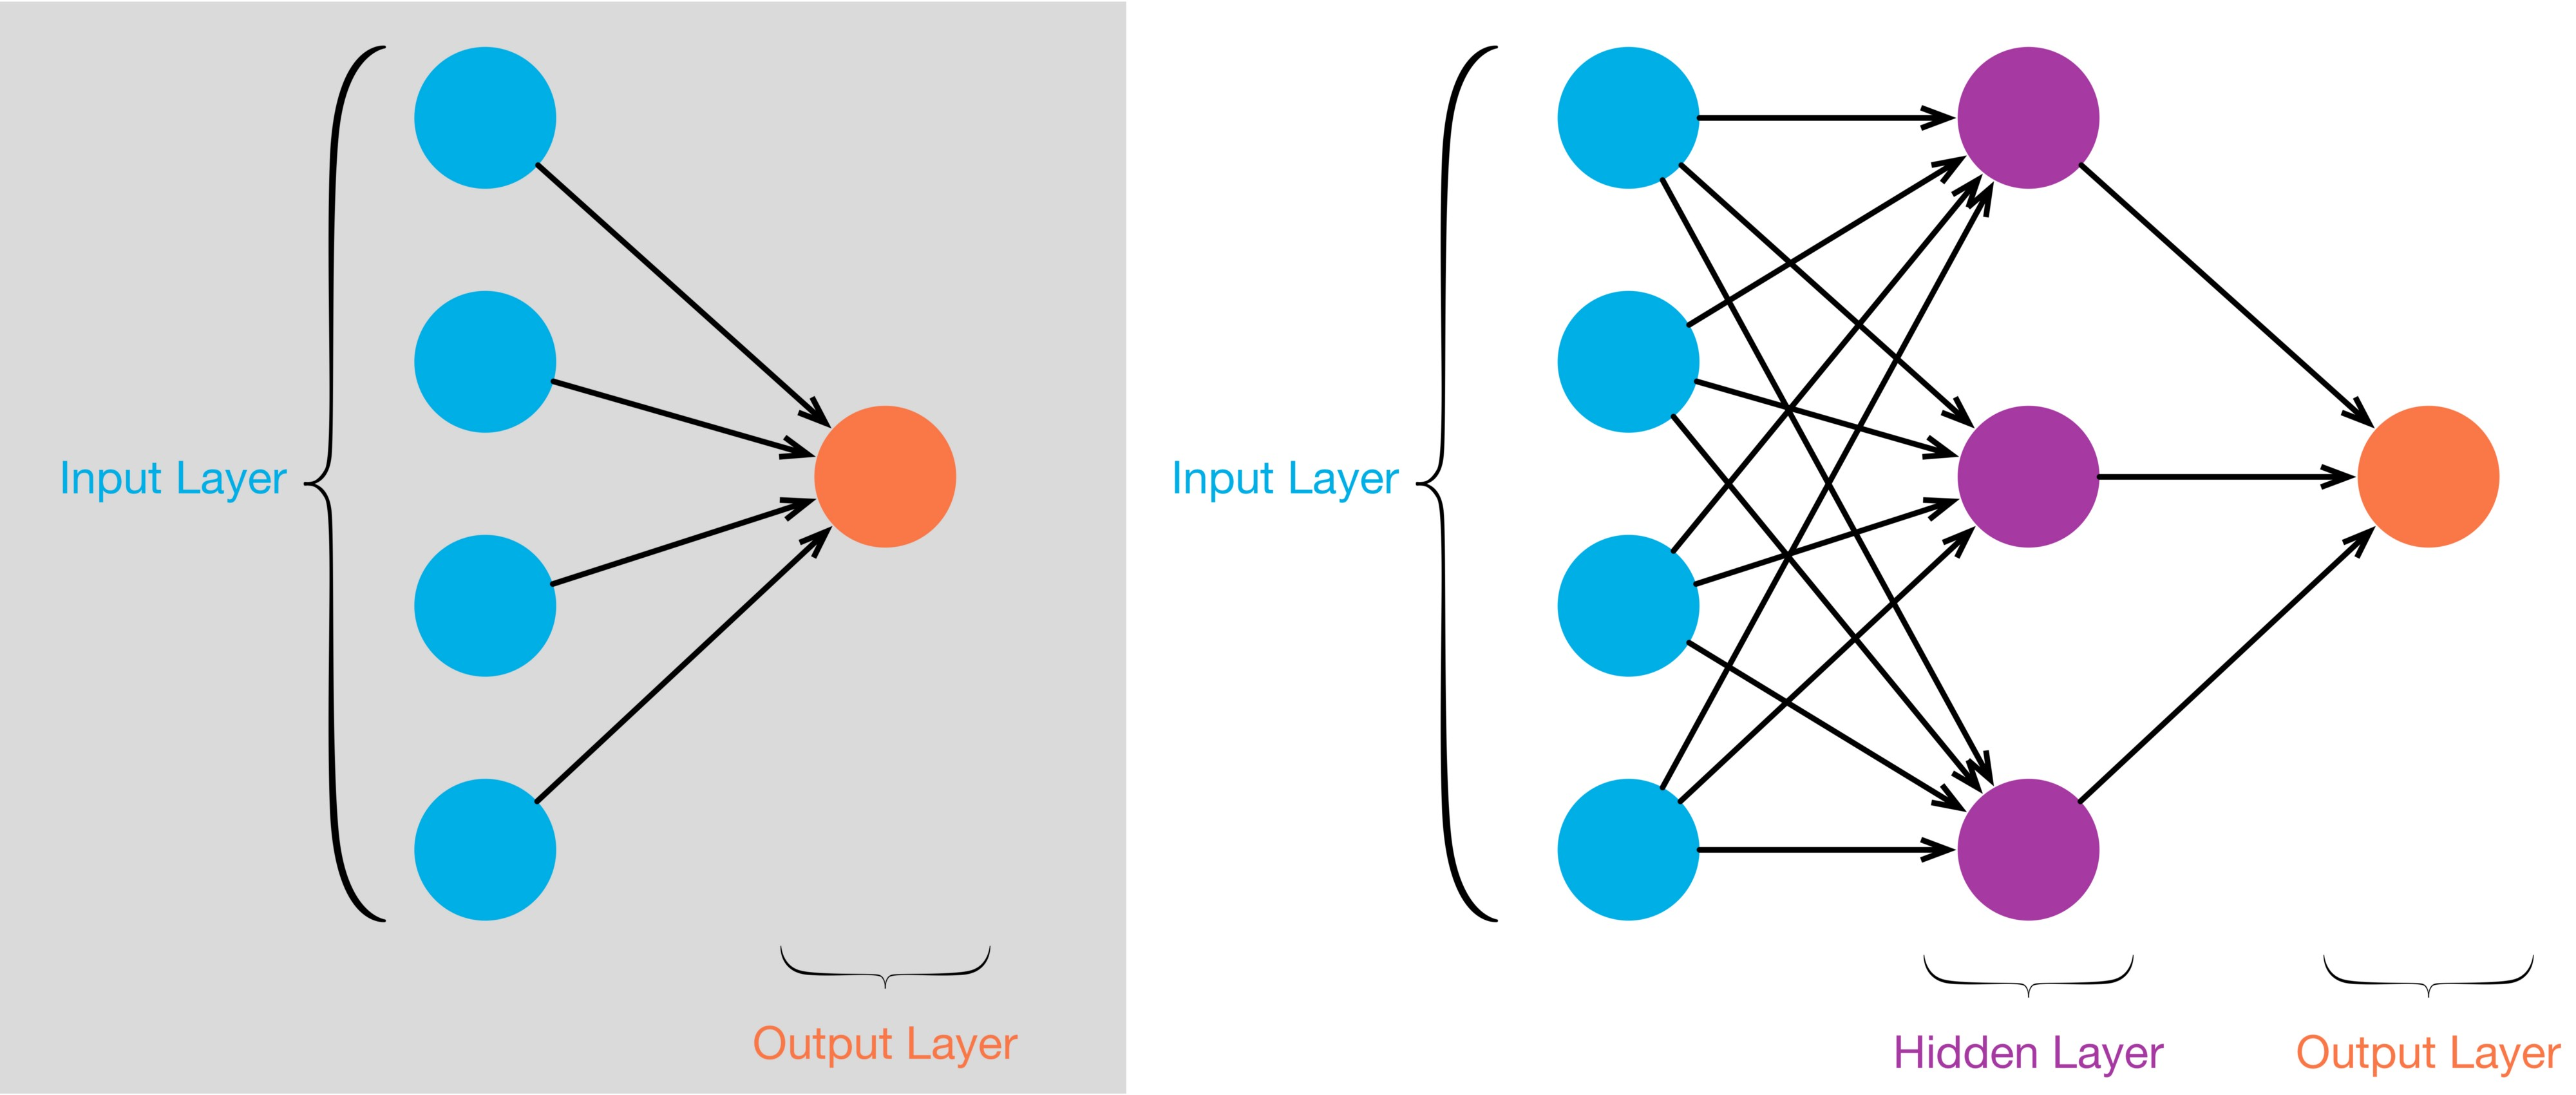
\includegraphics[scale=0.09]{img/nn-layers.jpeg}
\end{center}

Note that the input layer is usually ignored when counting the layers. \\

I won't give much details on the 1-layer, I strongly recommend Andrew Ng's tutorial for more details or this \href{https://towardsdatascience.com/everything-you-need-to-know-about-neural-networks-and-backpropagation-machine-learning-made-easy-e5285bc2be3a}{article} for a wrap up. \\

Let's now go into deeper details on the working on a 2-layer network.

\section{2-layer NN}
\section{Building the app}
\section{Deployment}

The deployment is done via \href{https://www.heroku.com/}{Heroku}. The clear steps for deployment are explained \href{https://dash.plotly.com/deployment}{here}. As mentioned in the link, "Heroku is one of the easiest platforms for deploying and managing public Flask applications.".

To sum up, the deployment consists in hosting the code in a Github repo, then deploying through Heroku with this command:

\lstset{language=bash}
\lstset{frame=lines}
\lstset{caption={Deploy the app}}
\lstset{label={lst:code_direct}}
\lstset{basicstyle=\footnotesize}
\begin{lstlisting}

$ git push heroku master

\end{lstlisting}


\vspace{5mm}
\section{Extensions}

The extension possibilities are endless! You can think about adding checkboxes/buttons so that the user can: \\

- the noise (standard deviation) associated with the data generation

- the number of data points to be generated

- the learning rate to be used during the parameter update

- the number of layers \\

For the last point however, I believe it would require significantly more work, especially if you don't use any neural network library (like tensorflow or pytorch) as we do here. \\

Have fun!
\section{Key insights}

When playing with the app we can already draw some interesting insights:

- 1 hidden unit gives a linear separation that is especially visible when selecting circles. \\

IMAGE \\

- 2 hidden units give a better separation \\

IMAGE \\

- 3 hidden units give a perfect separation of the clusters when choosing moons.

This illustrates the power of neural networks :) You can think of how good they can be when identifying human faces or finger prints!
\section{Conclusion}

This is my first article on Medium, I'd be happy to get your feedback with a clap and/or a comment. \\

Also, if there is not enough details in this article I can provide more.

\end{document} 
